\documentclass[a4paper,10pt]{article}
\usepackage[utf8]{inputenc}
\usepackage[margin=1.5cm, bottom=2cm]{geometry}
\usepackage{fancyhdr}
\usepackage{enumitem}
\usepackage{xcolor}
\usepackage{makeidx}
\usepackage[most]{tcolorbox}
\newtcolorbox{osservazioni}{
  colback=gray!8,    % sfondo grigio chiaro
  colframe=white,      % nessun bordo
  arc=2mm,            % angoli smussati
  boxrule=0pt,        % spessore bordo 0
  fontupper=\footnotesize,
  left=2mm, right=2mm, top=2mm, bottom=2mm,
  before skip=7pt,   % niente spazio prima
  after skip=15pt     % niente spazio dopo
}
\newtcolorbox{osservazioni2}{
  colback=gray!8,    % sfondo grigio chiaro
  colframe=white,      % nessun bordo
  arc=2mm,            % angoli smussati
  boxrule=0pt,        % spessore bordo 0
  fontupper=\small,
  left=5mm, right=5mm, top=3mm, bottom=3mm,
  before skip=0pt,   % niente spazio prima
  after skip=30pt     % niente spazio dopo
}
\pagestyle{fancy}
\usepackage{tikz}
\usetikzlibrary{automata, positioning}
\pagestyle{fancy}

\usepackage{makeidx}

%%%%%%%%%%%%%%%%%%%
\newcommand{\EsercitazioneNum}{04}
\newcommand{\Data}{14/10/2025}
\newcommand{\DocType}{Esercitazione} % o "Eserciziario"
\newcommand{\FullTitle}{\DocType\ \EsercitazioneNum}

\newcommand{\Header}{
\noindent
  \small \textbf{Computabilità, Complessità e Logica - a.a. 2025/26} \hfill \textbf{\FullTitle} \\[0.2cm]
  \scriptsize Matteo Liotta, \texttt{matteo.liotta@studenti.units.it} \hfill \Data \\[0.2cm]
  \noindent\makebox[\linewidth]{\rule{\linewidth}{0.4pt}} \\[0.3cm]}

\newcommand{\NewPageHeader}{
  \vfill
  \noindent\makebox[\linewidth]{\rule{\linewidth}{0.4pt}}
  \newpage
  {\Header}
}
%%%%%%%%%%%%%%%%%%%

% Numero di pagina in basso al centro
\fancyhf{}
\fancyfoot[C] \thepage
\renewcommand{\footrulewidth}{0pt} % niente linea in basso
\renewcommand{\headrulewidth}{0pt} % niente linea in alto

\begin{document}

\footnotesize  % font generale più piccolo
\Header\\[0.7cm]


%%%%%%%%%%%%%%%% FOGLIO 4

%% INDEX
\addcontentsline{toc}{section}{Esercitazione 04: \textit{Espressioni regolari e linguaggi regolari}} 
%%
\noindent\Large \textbf{Esercitazione 04}: \textit{Espressioni regolari e linguaggi regolari}
\begin{osservazioni}
    \textbf{\textit{Nota}}. Sono indicati in \textcolor{blue}{\textit{blu}} gli esercizi che non saranno trattati durante l'esercitazione, bensì lasciati come strumento aggiuntivo di esercitazione individuale. Resta comunque assoluta disponibilità per la loro risoluzione negli incontri successivi, qualora necessario.
\end{osservazioni}

{\normalsize
\begin{itemize}[label=, leftmargin=0pt]


    \item \underline{\textit{\textbf{Scrittura dell'espressione regolare equivalente ad un automa regolare}}}


    %% INDEX
    \addcontentsline{toc}{subsection}{Esercizio 30.} 
    %%
    \item \textbf{Esercizio 30. (**)}\\ Si consideri il seguente automa regolare definito su $\Sigma =\{a,b\}$. Si individui l'espressione regolare corrispondente, indicando chiaramente i passi intermedi.
    {
    \small
    \begin{center}
	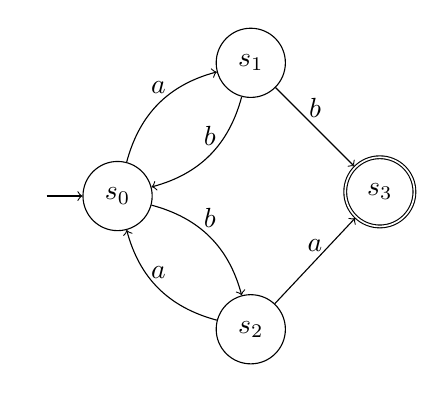
\begin{tikzpicture}
		\node[state, initial, initial text=] (A) {$s_0$};
		\node[state] (B) [above right=1.5of A] {$s_1$};
		\node[state] (C) [below right=1.5of A] {$s_2$};
		\node[state, accepting] (D) [below right=of B] {$s_3$};
		
		\path[->] 
        (A) edge[above, bend left] node{$a$} (B)
		(B) edge[above] node{$b$} (D)
		(A) edge[above, bend left] node{$b$} (C)
		(C) edge[above] node{$a$} (D)
		(B) edge[above, bend left] node{$b$} (A)
		(C) edge[above, bend left] node{$a$} (A);
    \end{tikzpicture}
    \end{center}
    }

    \begin{osservazioni}
        \underline{\textit{Soluzione.}}\\
        Si considerano i seguenti passaggi in cui viene preservata l'uguaglianza relativa al linguaggio accettato.
           {
    \small
    \begin{center}
	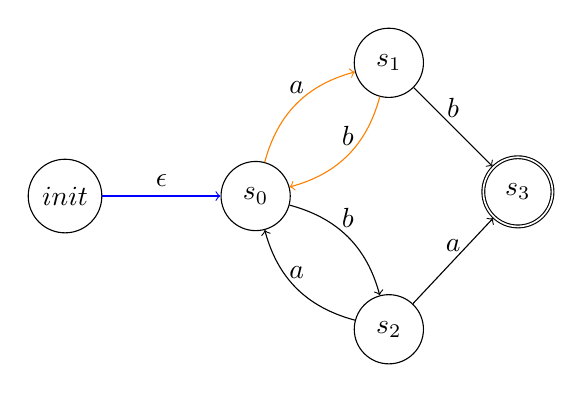
\begin{tikzpicture}
		
        \node[state, text=] (A) {$s_0$};
        \node[state, initial text=, left=1.5of A] (init) {$init$};
		\node[state] (B) [above right=1.5of A] {$s_1$};
		\node[state] (C) [below right=1.5of A] {$s_2$};
		\node[state,accepting] (D) [below right=of B] {$s_3$};

		
		\path[->] 
        (init) edge[above, draw=blue] node{$\epsilon$} (A)
        (A) edge[above, bend left, draw=orange] node{$a$} (B)
		(B) edge[above] node{$b$} (D)
		(A) edge[above, bend left] node{$b$} (C)
		(C) edge[above] node{$a$} (D)
		(B) edge[above, draw=orange, bend left] node{$b$} (A)
		(C) edge[above, bend left] node{$a$} (A);
    \end{tikzpicture}
    \end{center}
    }

 %%%2
           {
    \small
    \begin{center}
	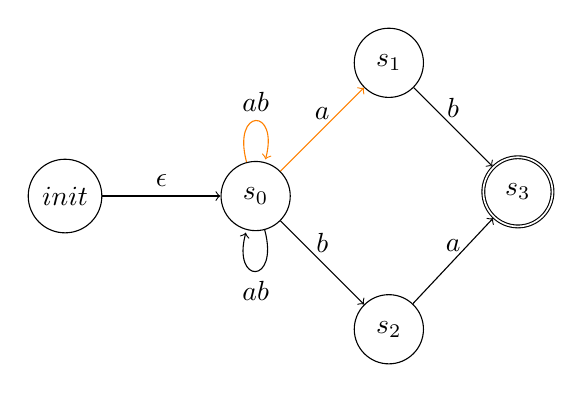
\begin{tikzpicture}
		
        \node[state, text=] (A) {$s_0$};
        \node[state, initial text=, left=1.5of A] (init) {$init$};
		\node[state] (B) [above right=1.5of A] {$s_1$};
		\node[state] (C) [below right=1.5of A] {$s_2$};
		\node[state,accepting] (D) [below right=of B] {$s_3$};

		
		\path[->] 
        (init) edge[above] node{$\epsilon$} (A)
        (A) edge[above, draw=orange] node{$a$} (B)
		(B) edge[above, draw=black] node{$b$} (D)
		(A) edge[above, draw=black] node{$b$} (C)
		(C) edge[above] node{$a$} (D)
        (A) edge[loop above, draw=orange] node{$ab$} (A)
        (A) edge[loop below, draw=black] node{$ab$} (A);
    \end{tikzpicture}
    \end{center}
    }

          {
    \small
    \begin{center}
	\begin{tikzpicture}
		
        \node[state, text=] (A) {$s_0$};
        \node[state, initial text=, left=1.5of A] (init) {$init$};
		\node[state,accepting] (D) [below right=of B] {$s_3$};

		
		\path[->] 
        (init) edge[above] node{$\epsilon$} (A)
        (A) edge[bend left, above] node{$ab$} (D)
		(A) edge[bend right, above] node{$ba$} (D)
        (A) edge[loop above] node{$(ab)^*+(ba)^*$} (A);
    \end{tikzpicture}
    \end{center}
    }
    Da cui: $$(ab)^* +(ba)^*(ab+ba)$$
    
    \end{osservazioni}


    \NewPageHeader


    %% INDEX
    \addcontentsline{toc}{subsection}{Esercizio 31.} 
    %%
    \item \textbf{\textcolor{blue}{Esercizio 31. (**)}}\\ Si consideri il seguente automa regolare definito su $\Sigma =\{a,b\}$. Si individui l'espressione regolare corrispondente, indicando chiaramente i passi intermedi.

    {
    \small
    \begin{center}
	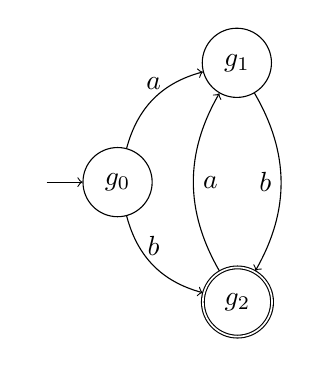
\begin{tikzpicture}
    	\node[state, initial, initial text=] (A) {$g_0$};
    	\node[state] (B) [above right=1.25of A] {$g_1$};
    	\node[state, accepting] (C) [below right=1.25of A] {$g_2$};
    %	\node[state, accepting] (D1) [right=of B] {$g_3$};
    %	\node[state, accepting] (D2) [right=of C] {$g_4$};
    %		
    	\path[->] (A) edge[above, bend left] node{$a$} (B)
    	 (B) edge[left, bend left] node{$b$} (C)
      (A) edge[above, bend right] node{$b$} (C)
      (C) edge[right, bend left] node{$a$} (B);
    %	\draw (D1) edge[above, bend left] node{$a$} (B);
    %	\draw (D2) edge[above, bend left] node{$b$} (C);
    
    \end{tikzpicture}
    \end{center}
    }
      \begin{osservazioni}
        \underline{\textit{Soluzione.}}\\
        Si considerano i seguenti passaggi in cui viene preservata l'uguaglianza relativa al linguaggio accettato.



    {
    \small
    \begin{center}
	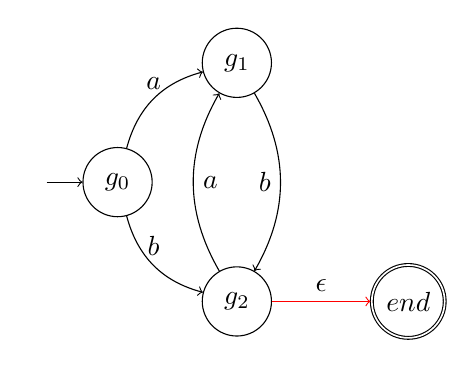
\begin{tikzpicture}
    	\node[state, initial, initial text=] (A) {$g_0$};
    	\node[state] (B) [above right=1.25of A] {$g_1$};
    	\node[state] (C) [below right=1.25of A] {$g_2$};
        \node[state, accepting] (D) [right=1.25of C] {$end$};

    %	\node[state, accepting] (D1) [right=of B] {$g_3$};
    %	\node[state, accepting] (D2) [right=of C] {$g_4$};
    %		
    	\path[->] (A) edge[above, bend left] node{$a$} (B)
    	 (B) edge[left, bend left] node{$b$} (C)
      (A) edge[above, bend right] node{$b$} (C)
      (C) edge[right, bend left] node{$a$} (B)
      (C) edge[above, draw=red] node{$\epsilon$} (D);
    %	\draw (D1) edge[above, bend left] node{$a$} (B);
    %	\draw (D2) edge[above, bend left] node{$b$} (C);
    
    \end{tikzpicture}
    \end{center}
    }

    {
    \small
    \begin{center}
	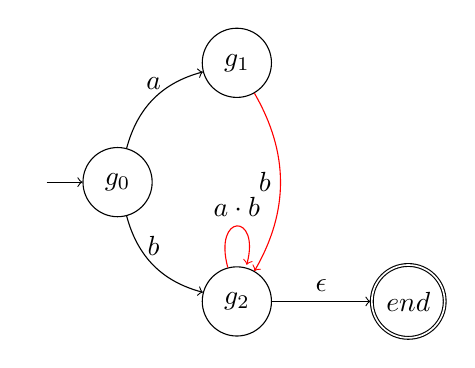
\begin{tikzpicture}
    	\node[state, initial, initial text=] (A) {$g_0$};
    	\node[state] (B) [above right=1.25of A] {$g_1$};
    	\node[state] (C) [below right=1.25of A] {$g_2$};
        \node[state, accepting] (D) [right=1.25of C] {$end$};
    %	\node[state, accepting] (D1) [right=of B] {$g_3$};
    %	\node[state, accepting] (D2) [right=of C] {$g_4$};
    %		
    	\path[->] (A) edge[above, bend left] node{$a$} (B)
    	 (B) edge[left, bend left, draw=red] node{$b$} (C)
      (A) edge[above, bend right] node{$b$} (C)
      (C) edge[above, loop above, draw=red] node{$a\cdot b$} (C)
      (C) edge[above, draw=black] node{$\epsilon$} (D);

    %	\draw (D1) edge[above, bend left] node{$a$} (B);
    %	\draw (D2) edge[above, bend left] node{$b$} (C);
    
    \end{tikzpicture}
    \end{center}
    }


    {
    \small
    \begin{center}
	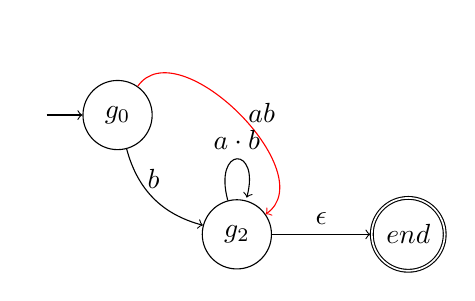
\begin{tikzpicture}
    	\node[state, initial, initial text=] (A) {$g_0$};
    	\node[state] (C) [below right=1.25of A] {$g_2$};
        \node[state, accepting] (D) [right=1.25of C] {$end$};
    %	\node[state, accepting] (D1) [right=of B] {$g_3$};
    %	\node[state, accepting] (D2) [right=of C] {$g_4$};
    %		
    	\path[->] 
      (A) edge[right, bend left=100, draw=red] node{$ab$} (C)
      (A) edge[above, bend right] node{$b$} (C)
      (C) edge[above, loop above, draw=black] node{$a\cdot b$} (C)
      (C) edge[above, draw=black] node{$\epsilon$} (D);

    %	\draw (D1) edge[above, bend left] node{$a$} (B);
    %	\draw (D2) edge[above, bend left] node{$b$} (C);

    
    \end{tikzpicture}
    \end{center}
    }

        {
    \small
    \begin{center}
	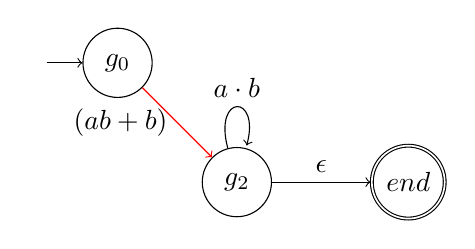
\begin{tikzpicture}
    	\node[state, initial, initial text=] (A) {$g_0$};
        \node[state] (C) [below right=1.25of A] {$g_2$};
        \node[state, accepting] (D) [right=1.25of C] {$end$};    %	\node[state, accepting] (D1) [right=of B] {$g_3$};
    %	\node[state, accepting] (D2) [right=of C] {$g_4$};
    %		
    	\path[->] 
      (A) edge[left, draw = red] node{$(ab +b)$} (C)
      (C) edge[above, loop above, draw=black] node{$a\cdot b$} (C)
      (C) edge[above, draw=black] node{$\epsilon$} (D);

    %	\draw (D1) edge[above, bend left] node{$a$} (B);
    %	\draw (D2) edge[above, bend left] node{$b$} (C);
    
    \end{tikzpicture}
    \end{center}
    }
    Da cui:
    $$(ab+b) (ab)^*$$
    \end{osservazioni}

    \NewPageHeader

    %% INDEX
    \addcontentsline{toc}{subsection}{Esercizio 32.} 
    %%
    \item \textbf{Esercizio 32. (**)}\\ Si consideri il seguente automa regolare definito su $\Sigma =\{a,b\}$. Si individui l'espressione regolare corrispondente, indicando chiaramente i passi intermedi.

    {
    \small

\begin{center}
	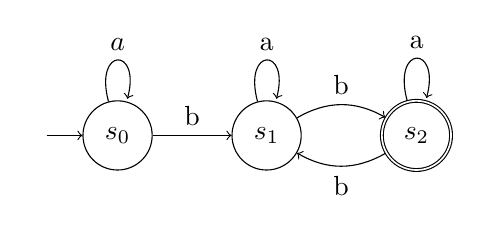
\begin{tikzpicture}
        \node[state, initial, initial text=] (A) {$s_0$};
        \node[state, right= of A] (B) {$s_1$};
        \node[state, accepting, right= of B] (C) {$s_2$};
%	
		\path[->] 
        (A) edge [loop above] node{$a$} (A)
            edge [above] node{b} (B)
        (B) edge [loop above] node{a} (B)
            edge [bend left, above] node{b} (C)
        (C) edge [bend left, below] node{b} (B)
            edge [loop above] node{a} (C);
            
        
	\end{tikzpicture}
\end{center}
    }

    \begin{osservazioni}
        \underline{\textit{Soluzione.}}\\
Si considerano i seguenti passaggi in cui viene preservata l'uguaglianza relativa al linguaggio accettato.



    {
    \small

\begin{center}
	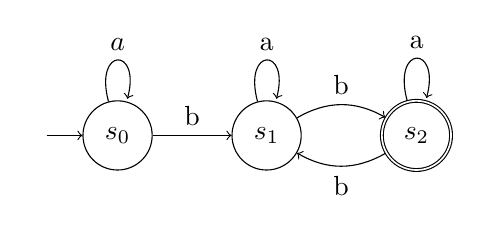
\begin{tikzpicture}
        \node[state, initial, initial text=] (A) {$s_0$};
        \node[state, right= of A] (B) {$s_1$};
        \node[state, accepting, right= of B] (C) {$s_2$};
%	
		\path[->] 
        (A) edge [loop above] node{$a$} (A)
            edge [above] node{b} (B)
        (B) edge [loop above] node{a} (B)
            edge [bend left, above] node{b} (C)
        (C) edge [bend left, below] node{b} (B)
            edge [loop above] node{a} (C);
            
        
	\end{tikzpicture}
\end{center}
    }


        {
    \small

\begin{center}
	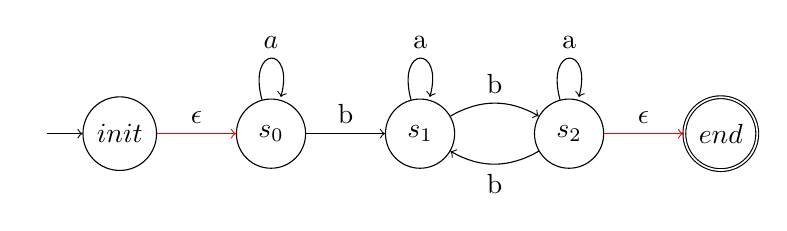
\begin{tikzpicture}
        \node[state, initial, initial text=] (init) {$init$};
        \node[state, right= of init] (A) {$s_0$};
        \node[state, right= of A] (B) {$s_1$};
        \node[state, right= of B] (C) {$s_2$};
        \node[state, accepting, right= of C] (end) {$end$};
%	
		\path[->] 
        (init) edge [above, draw=red] node{$\epsilon$} (A)
        (A) edge [loop above] node{$a$} (A)
            edge [above] node{b} (B)
        (B) edge [loop above] node{a} (B)
            edge [bend left, above] node{b} (C)
        (C) edge [bend left, below] node{b} (B)
            edge [loop above] node{a} (C)
            edge [above, draw=red] node{$\epsilon$} (end);
            
        
	\end{tikzpicture}
\end{center}
    }

            {
    \small

\begin{center}
	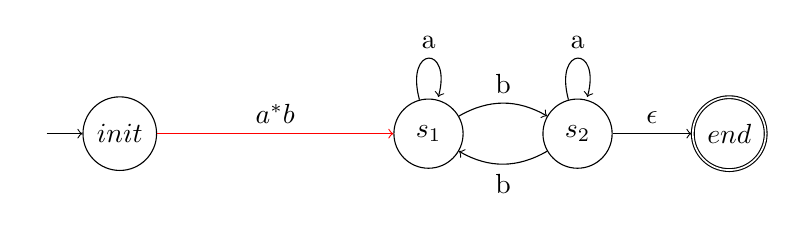
\begin{tikzpicture}
        \node[state, initial, initial text=] (init) {$init$};
        \node[state, right=3 of init] (B) {$s_1$};
        \node[state, right= of B] (C) {$s_2$};
        \node[state, accepting, right= of C] (end) {$end$};
%	
		\path[->] 
        (init)
            edge [above, draw=red] node{$a^*b$} (B)
        (B) edge [loop above] node{a} (B)
            edge [bend left, above] node{b} (C)
        (C) edge [bend left, below] node{b} (B)
            edge [loop above] node{a} (C)
            edge [above, draw=black] node{$\epsilon$} (end);
            
        
	\end{tikzpicture}
\end{center}
    }

            {
    \small

\begin{center}
	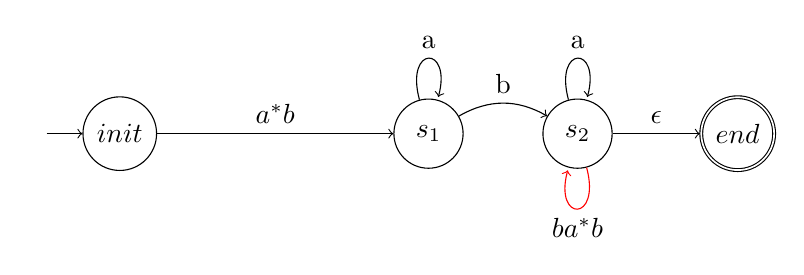
\begin{tikzpicture}
        \node[state, initial, initial text=] (init) {$init$};
        \node[state, right=3 of init] (B) {$s_1$};
        \node[state, right= of B] (C) {$s_2$};
        \node[state, accepting, right=3 of B] (end) {$end$};
%	
		\path[->] 
        (init)
            edge [above, draw=black] node{$a^*b$} (B)
        (B) edge [loop above] node{a} (B)
            edge [bend left, above] node{b} (C)
        (C) edge [loop below,below, draw=red] node{$ba^*b$} (C)
        %(C) edge [bend left, below] node{b} (B)
        (C) edge [loop above] node{a} (C)
            edge [above, draw=black] node{$\epsilon$} (end);
            
        
	\end{tikzpicture}
\end{center}
    }

            {
    \small

\begin{center}
	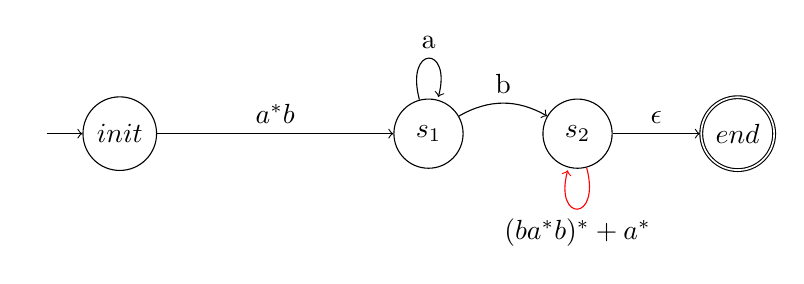
\begin{tikzpicture}
        \node[state, initial, initial text=] (init) {$init$};
        \node[state, right=3 of init] (B) {$s_1$};
        \node[state, right= of B] (C) {$s_2$};
        \node[state, accepting, right=3 of B] (end) {$end$};
%	
		\path[->] 
        (init)
            edge [above, draw=black] node{$a^*b$} (B)
        (B) edge [loop above] node{a} (B)
            edge [bend left, above] node{b} (C)
        (C) edge [loop below,below, draw=red] node{$(ba^*b)^*+a^*$} (C)
        %(C) edge [bend left, below] node{b} (B)
        (C) %edge [loop above] node{a} (C)
            edge [above, draw=black] node{$\epsilon$} (end);
            
        
	\end{tikzpicture}
\end{center}
    }

            {
    \small

\begin{center}
	\begin{tikzpicture}
        \node[state, initial, initial text=] (init) {$init$};
        %\node[state, right=3 of init] (B) {$s_1$}
        \node[state, right=5 of init] (C) {$s_2$};
        \node[state, accepting, right=3 of B] (end) {$end$};
%	
		\path[->] 
        (init)
            %edge [above, draw=black] node{$a^*b$} (B)
            edge [above] node{$a^*ba^*b$} (C)
            %edge [loop below,below, draw=red] node{$(a^*ba^*b)+a$} (C)
        %(C) edge [bend left, below] node{b} (B)
        (C) edge [loop above] node{$(ba^*b)^*+a^*$} (C)
            edge [above, draw=black] node{$\epsilon$} (end);
        
        
	\end{tikzpicture}
\end{center}
    }

    Da cui:
    $$a^*ba^*b \bigg( (ba^*b)^*+a^* \bigg)^*$$
    

    \end{osservazioni}


    \NewPageHeader

    %% INDEX
    \addcontentsline{toc}{subsection}{Esercizio 33.} 
    %%
    \item \textbf{\textcolor{blue}{Esercizio 33. (*)}}\\ Si consideri il seguente automa regolare definito su $\Sigma =\{a,b\}$. Si individui l'espressione regolare corrispondente, indicando chiaramente i passi intermedi.
    {
    \small
    \begin{center}
    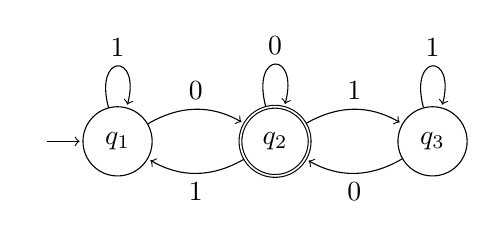
\begin{tikzpicture}[shorten >=1pt, node distance=2cm, on grid, auto]
        \node[state, initial, initial text=] (q1)   {$q_1$};
        \node[state, accepting] (q2) [right=of q1] {$q_2$};
        \node[state] (q3) [right=of q2] {$q_3$};
        
        \path[->]
        (q1) edge [bend left] node {0} (q2)
             edge [loop above] node {1} ()
        (q2) edge [loop above] node {0} ()
             edge [bend left] node {1} (q3)
             edge [bend left] node {1} (q1)
        (q3) edge [loop above] node {1} ()
             edge [bend left] node {0} (q2);
         
    \end{tikzpicture}
    \end{center}
    }

        \begin{osservazioni}
        \underline{\textit{Soluzione.}}\\
        L'automa riconosce il linguaggio identificato da $$1^*0\bigg(0^*+(1^+0)^*\bigg)^*$$
    \end{osservazioni}
$\\$

    \item \underline{\textit{\textbf{Identificazione del linguaggio regolare definito da una espressione regolare}}}

        %% INDEX
    \addcontentsline{toc}{subsection}{Esercizio 34.} 
    %%
    \item \textbf{Esercizio 34. (**)}\\ Si consideri la seguente espressione regolare su $\Sigma=\{a,b,\#\}$
    {\begin{center}
        $\bigg((T\cdot R)^* \cdot \#\bigg)^*$
    \end{center}} 
    dove:
    \begin{itemize}[label=]
        \item $T=\{b^k:\leq 4\}$
        \item $R =\{a^2, a^4, a^6\}$
    \end{itemize}
    Si indichi il linguaggio definito dall'espressione regolare in questione.\\
        \begin{osservazioni}
        \underline{\textit{Soluzione.}}\\
    L'automa che riconosce il linguaggio è ottenuto attraverso i seguenti passaggi modulari:\\

    \textbf{1. L'automa che riconosce il linguaggio identificato da $T$}
        {
    \small
    \begin{center}
    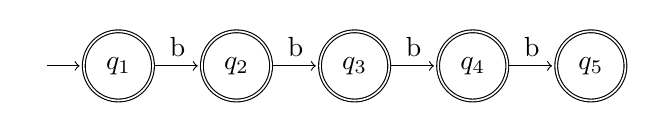
\begin{tikzpicture}[shorten >=1pt, node distance=2cm, on grid, auto]
        \node[state, accepting, initial, initial text=] (q1)   {$q_1$};
        \node[state, accepting] (q2) [right=1.5of q1] {$q_2$};
        \node[state, accepting] (q3) [right=1.5of q2] {$q_3$};
        \node[state, accepting] (q4) [right=1.5of q3] {$q_4$};
        \node[state, accepting] (q5) [right=1.5of q4] {$q_5$};

     
        \path[->]
        (q1) edge node {b} (q2)
        (q2) edge node {b} (q3)
        (q3) edge node {b} (q4)
        (q4) edge node {b} (q5);

         
    \end{tikzpicture}
    \end{center}
    }

  \textbf{2. L'automa che riconosce il linguaggio identificato da $R$}
        {
    \small
    \begin{center}
    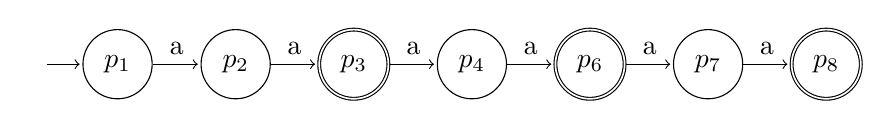
\begin{tikzpicture}[shorten >=1pt, node distance=2cm, on grid, auto]
        \node[state, initial, initial text=] (p1)   {$p_1$};
        \node[state] (p2) [right=1.5of p1] {$p_2$};
        \node[state, accepting] (p3) [right=1.5of p2] {$p_3$};
        \node[state] (p4) [right=1.5of p3] {$p_4$};
        \node[state, accepting] (p5) [right=1.5of p4] {$p_6$};
        \node[state] (p6) [right=1.5of p5] {$p_7$};
        \node[state, accepting] (p7) [right=1.5of p6] {$p_8$};

     
        \path[->]
        (p1) edge node {a} (p2)
        (p2) edge node {a} (p3)
        (p3) edge node {a} (p4)
        (p4) edge node {a} (p5)
        (p5) edge node {a} (p6)
        (p6) edge node {a} (p7);
         
    \end{tikzpicture}
    \end{center}
    }

    
    \textbf{3. L'automa che riconosce il linguaggio identificato da $T\cdot R$}
        {
    \small
    \begin{center}
    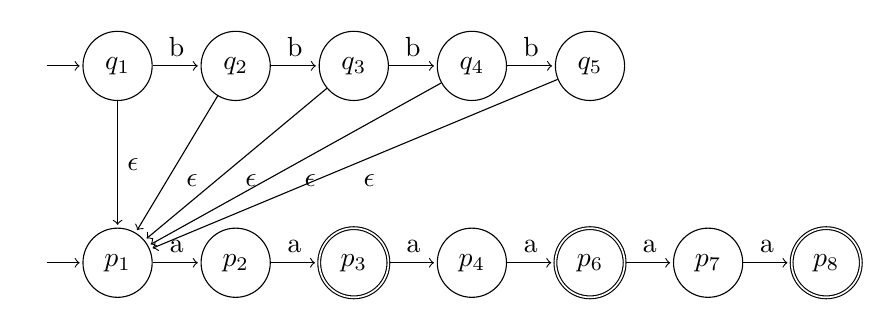
\begin{tikzpicture}[shorten >=1pt, node distance=2cm, on grid, auto]
        \node[state, initial, initial text=] (q1)   {$q_1$};
        \node[state] (q2) [right=1.5of q1] {$q_2$};
        \node[state] (q3) [right=1.5of q2] {$q_3$};
        \node[state] (q4) [right=1.5of q3] {$q_4$};
        \node[state] (q5) [right=1.5of q4] {$q_5$};

        \node[state, below=2.5of q1, initial, initial text=] (p1)   {$p_1$};
        \node[state] (p2) [right=1.5of p1] {$p_2$};
        \node[state, accepting] (p3) [right=1.5of p2] {$p_3$};
        \node[state] (p4) [right=1.5of p3] {$p_4$};
        \node[state, accepting] (p5) [right=1.5of p4] {$p_6$};
        \node[state] (p6) [right=1.5of p5] {$p_7$};
        \node[state, accepting] (p7) [right=1.5of p6] {$p_8$};

     
        \path[->]
        (q1) edge node {b} (q2)
        (q2) edge node {b} (q3)
        (q3) edge node {b} (q4)
        (q4) edge node {b} (q5)
        
        (q1) edge node {$\epsilon$} (p1)
        (q2) edge node {$\epsilon$} (p1)
        (q3) edge node {$\epsilon$} (p1)
        (q4) edge node {$\epsilon$} (p1)
        (q5) edge node {$\epsilon$} (p1)

        (p1) edge node {a} (p2)
        (p2) edge node {a} (p3)
        (p3) edge node {a} (p4)
        (p4) edge node {a} (p5)
        (p5) edge node {a} (p6)
        (p6) edge node {a} (p7);
         
    \end{tikzpicture}
    \end{center}
    }
    
    \end{osservazioni}
    \NewPageHeader
    \begin{osservazioni}
    
    \textbf{3. L'automa che riconosce il linguaggio identificato da $(T\cdot R)^*$}
        {
    \small
    \begin{center}
    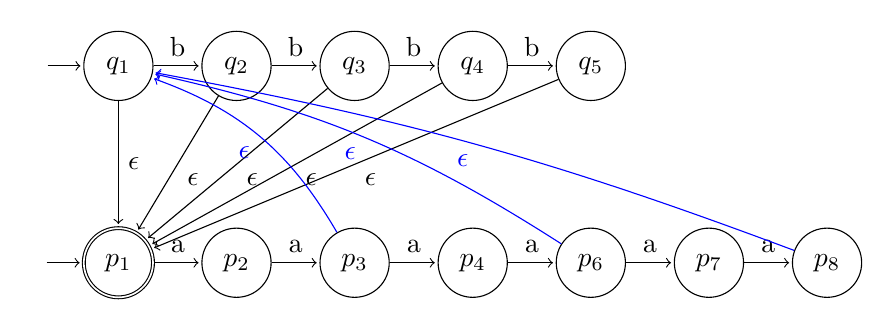
\begin{tikzpicture}[shorten >=1pt, node distance=2cm, on grid, auto]
        \node[state, initial, initial text=] (q1)   {$q_1$};
        \node[state] (q2) [right=1.5of q1] {$q_2$};
        \node[state] (q3) [right=1.5of q2] {$q_3$};
        \node[state] (q4) [right=1.5of q3] {$q_4$};
        \node[state] (q5) [right=1.5of q4] {$q_5$};

        \node[state, accepting, below=2.5of q1, initial, initial text=] (p1)   {$p_1$};
        \node[state] (p2) [right=1.5of p1] {$p_2$};
        \node[state, ] (p3) [right=1.5of p2] {$p_3$};
        \node[state] (p4) [right=1.5of p3] {$p_4$};
        \node[state, ] (p5) [right=1.5of p4] {$p_6$};
        \node[state] (p6) [right=1.5of p5] {$p_7$};
        \node[state, ] (p7) [right=1.5of p6] {$p_8$};

     
        \path[->]
        (q1) edge node {b} (q2)
        (q2) edge node {b} (q3)
        (q3) edge node {b} (q4)
        (q4) edge node {b} (q5)
        
        (q1) edge node {$\epsilon$} (p1)
        (q2) edge node {$\epsilon$} (p1)
        (q3) edge node {$\epsilon$} (p1)
        (q4) edge node {$\epsilon$} (p1)
        (q5) edge node {$\epsilon$} (p1)

        (p1) edge node {a} (p2)
        (p2) edge node {a} (p3)
        (p3) edge node {a} (p4)
        (p4) edge node {a} (p5)
        (p5) edge node {a} (p6)
        (p6) edge node {a} (p7)

        (p3) edge [bend right=20, draw=blue] node[blue] {$\epsilon$} (q1)
        (p5) edge [bend right=10, draw=blue] node[blue] {$\epsilon$} (q1)
        (p7) edge [bend right=5, draw=blue] node[blue] {$\epsilon$} (q1);
         
    \end{tikzpicture}
    \end{center}
    }

    
    \textbf{3. L'automa che riconosce il linguaggio identificato da $(T\cdot R)^*\#$}
        {
    \small
    \begin{center}
    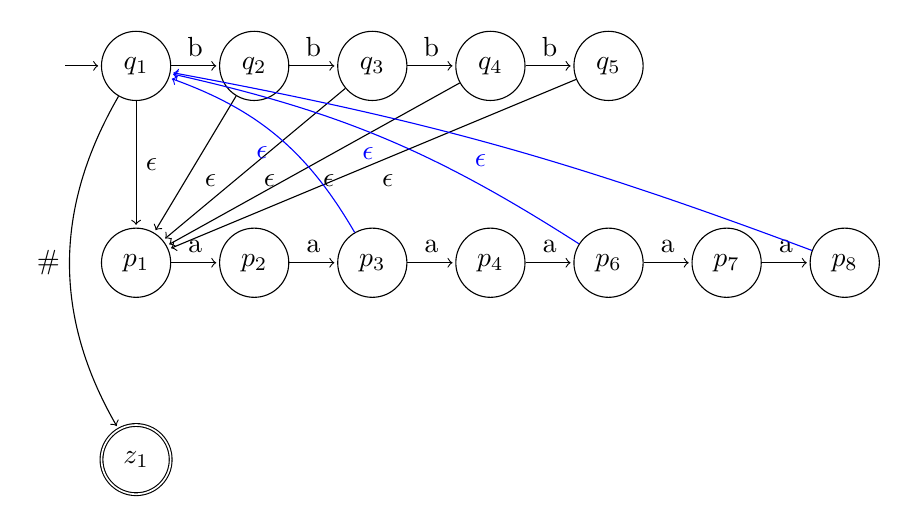
\begin{tikzpicture}[shorten >=1pt, node distance=2cm, on grid, auto]
        \node[state, initial, initial text=] (q1)   {$q_1$};
        \node[state] (q2) [right=1.5of q1] {$q_2$};
        \node[state] (q3) [right=1.5of q2] {$q_3$};
        \node[state] (q4) [right=1.5of q3] {$q_4$};
        \node[state] (q5) [right=1.5of q4] {$q_5$};

        \node[state, below=2.5of q1, initial text=] (p1)   {$p_1$};
        \node[state] (p2) [right=1.5of p1] {$p_2$};
        \node[state, ] (p3) [right=1.5of p2] {$p_3$};
        \node[state] (p4) [right=1.5of p3] {$p_4$};
        \node[state, ] (p5) [right=1.5of p4] {$p_6$};
        \node[state] (p6) [right=1.5of p5] {$p_7$};
        \node[state, ] (p7) [right=1.5of p6] {$p_8$};

        \node[state, accepting, below=2.5of p1, initial text=] (z1)   {$z_1$};

     
        \path[->]
        (q1) edge node {b} (q2)
        (q2) edge node {b} (q3)
        (q3) edge node {b} (q4)
        (q4) edge node {b} (q5)
        
        (q1) edge node {$\epsilon$} (p1)
        (q2) edge node {$\epsilon$} (p1)
        (q3) edge node {$\epsilon$} (p1)
        (q4) edge node {$\epsilon$} (p1)
        (q5) edge node {$\epsilon$} (p1)

        (p1) edge node {a} (p2)
        (p2) edge node {a} (p3)
        (p3) edge node {a} (p4)
        (p4) edge node {a} (p5)
        (p5) edge node {a} (p6)
        (p6) edge node {a} (p7)

        (p3) edge [bend right=20, draw=blue] node[blue] {$\epsilon$} (q1)
        (p5) edge [bend right=10, draw=blue] node[blue] {$\epsilon$} (q1)
        (p7) edge [bend right=5, draw=blue] node[blue] {$\epsilon$} (q1)

        (q1) edge[bend right, left] node {$\#$} (z1);
         
    \end{tikzpicture}
    \end{center}
    }

    Dunque, l'automa finale:

        {
    \small
    \begin{center}
    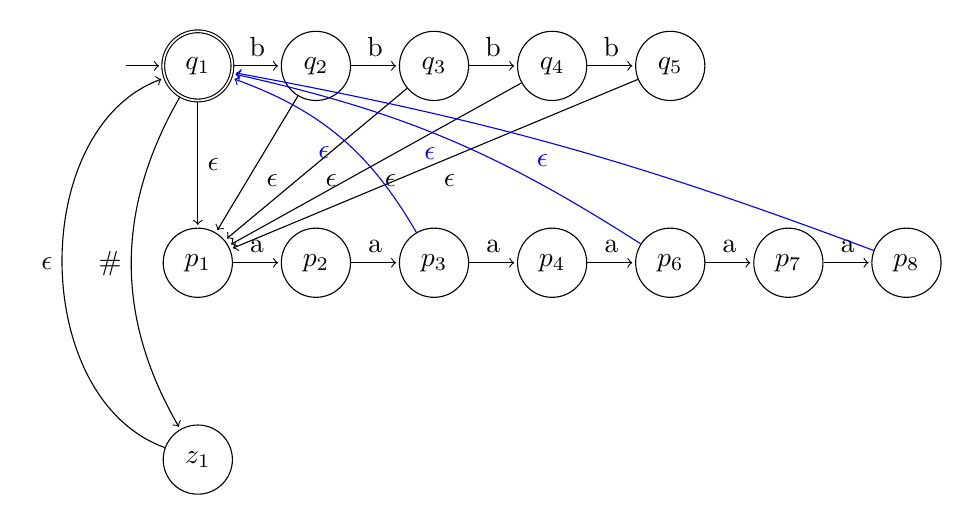
\begin{tikzpicture}[shorten >=1pt, node distance=2cm, on grid, auto]
        \node[state, accepting, initial, initial text=] (q1)   {$q_1$};
        \node[state] (q2) [right=1.5of q1] {$q_2$};
        \node[state] (q3) [right=1.5of q2] {$q_3$};
        \node[state] (q4) [right=1.5of q3] {$q_4$};
        \node[state] (q5) [right=1.5of q4] {$q_5$};

        \node[state, below=2.5of q1, initial text=] (p1)   {$p_1$};
        \node[state] (p2) [right=1.5of p1] {$p_2$};
        \node[state, ] (p3) [right=1.5of p2] {$p_3$};
        \node[state] (p4) [right=1.5of p3] {$p_4$};
        \node[state, ] (p5) [right=1.5of p4] {$p_6$};
        \node[state] (p6) [right=1.5of p5] {$p_7$};
        \node[state, ] (p7) [right=1.5of p6] {$p_8$};

        \node[state, below=2.5of p1, initial text=] (z1)   {$z_1$};

     
        \path[->]
        (q1) edge node {b} (q2)
        (q2) edge node {b} (q3)
        (q3) edge node {b} (q4)
        (q4) edge node {b} (q5)
        
        (q1) edge node {$\epsilon$} (p1)
        (q2) edge node {$\epsilon$} (p1)
        (q3) edge node {$\epsilon$} (p1)
        (q4) edge node {$\epsilon$} (p1)
        (q5) edge node {$\epsilon$} (p1)

        (p1) edge node {a} (p2)
        (p2) edge node {a} (p3)
        (p3) edge node {a} (p4)
        (p4) edge node {a} (p5)
        (p5) edge node {a} (p6)
        (p6) edge node {a} (p7)

        (p3) edge [bend right=20, draw=blue] node[blue] {$\epsilon$} (q1)
        (p5) edge [bend right=10, draw=blue] node[blue] {$\epsilon$} (q1)
        (p7) edge [bend right=5, draw=blue] node[blue] {$\epsilon$} (q1)

        (q1) edge[bend right, left] node {$\#$} (z1)
        (z1) edge [bend left=70] node {$\epsilon$} (q1);
         
    \end{tikzpicture}
    \end{center}
    }
    
    \end{osservazioni}

    
    \NewPageHeader
    %% INDEX
    \addcontentsline{toc}{subsection}{Esercizio 35.} 
    %%
    \item \textbf{Esercizio 35. (**)}\\ Si consideri la seguente espressione regolare su $\Sigma=\{a,b\}$
    {\begin{center}
        $\bigg( \quad \bigg((a+b)^*\cdot(bc+dc^*)\bigg) \cdot b\quad\bigg)^*$
    \end{center}} 
    Si costruisca l'automa regolare tale da riconoscere il linguaggio definito dall'espressione regolare proposta.\\

    \begin{osservazioni}
        \underline{\textit{Soluzione.}}\\
        Seguendo lo stesso procedimento evidenziato sopra, l'automa ottenuto è il seguente:


        {
    \small
    \begin{center}
    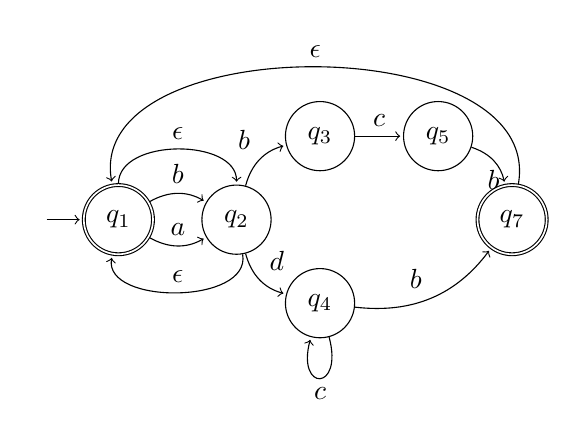
\begin{tikzpicture}[shorten >=1pt, node distance=2cm, on grid, auto]
        \node[state, accepting, initial, initial text=] (q1)   {$q_1$};
        \node[state] (q2) [right=1.5of q1] {$q_2$};
        \node[state] (q3) [above right=1.5of q2] {$q_3$};
        \node[state] (q4) [below right=1.5of q2] {$q_4$};
        \node[state] (q5) [right=1.5of q3] {$q_5$};
        %\node[state] (q6) [right=1.5of q4] {$q_6$};
        \node[state, accepting] (q7) [right=3.5of q2] {$q_7$};


     
        \path[->]
        (q1) edge [bend right] node {$a$} (q2)
        (q1) edge [bend left] node {$b$} (q2)
        (q2) edge [bend left=100, above] node {$\epsilon$} (q1)
        (q1) edge [bend left=90, above] node {$\epsilon$} (q2)
        
        
        (q2) edge [bend right] node {$d$} (q4)
        (q2) edge [bend left] node {$b$} (q3)

        (q3) edge node {$c$} (q5)
        (q4) edge [bend right=30] node {$b$} (q7)
        (q4) edge [loop below] node {$c$} (q4)
        %(q6) edge [loop below] node {$\epsilon$} (q6)
        
        (q5) edge [bend left, below]  node {$b$} (q7)
        %(q6) edge [bend right] node {$b$} (q7)
        (q7) edge [bend right=100, above] node {$\epsilon$} (q1);
        


         
    \end{tikzpicture}
    \end{center}
    }        
    \end{osservazioni}

    %% INDEX
    \addcontentsline{toc}{subsection}{Esercizio 36.} 
    %%
    \item \textbf{\textcolor{blue}{Esercizio 36. (**)}}\\ Si consideri la seguente espressione regolare su $\Sigma=\{a,b,\#\}$
    {\begin{center}
        $\bigg(\quad \bigg((a + b)\cdot (b +c)\bigg)^*\cdot (c + d)^*\quad \bigg)^*$
    \end{center}} 

    
    Si costruisca l'automa regolare tale da riconoscere il linguaggio definito dall'espressione regolare proposta.\\

   \begin{osservazioni}
        \underline{\textit{Soluzione.}}\\
        Seguendo lo stesso procedimento evidenziato sopra, l'automa ottenuto è il seguente:

    
        {
    \small
    \begin{center}
    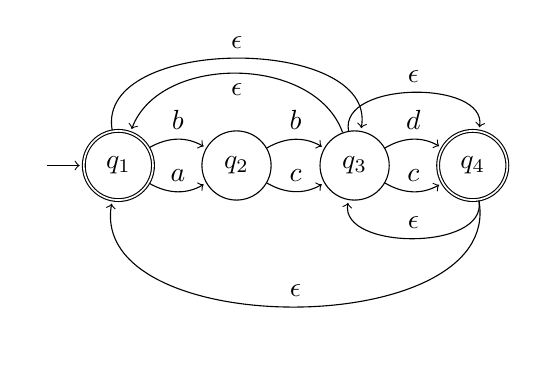
\begin{tikzpicture}[shorten >=1pt, node distance=2cm, on grid, auto]
        \node[accepting, state, initial, initial text=] (q1)   {$q_1$};
        \node[state] (q2) [right=1.5of q1] {$q_2$};
        \node[state] (q3) [right=1.5of q2] {$q_3$};
        \node[state, accepting] (q4) [right=1.5of q3] {$q_4$};




     
        \path[->]
        (q1) edge [bend right] node {$a$} (q2)
        (q1) edge [bend left] node {$b$} (q2)
        (q3) edge [bend right=70, below] node {$\epsilon$} (q1)
        (q1) edge [bend left=100, above] node {$\epsilon$} (q3)
        
        (q2) edge [bend right] node {$c$} (q3)
        (q2) edge [bend left] node {$b$} (q3)

        (q3) edge [bend right] node {$c$} (q4)
        (q3) edge [bend left=100] node {$\epsilon$} (q4)
        (q3) edge [bend left] node {$d$} (q4)
        (q4) edge [bend left=100, above] node {$\epsilon$} (q3)
        (q4) edge [bend left=100, above] node {$\epsilon$} (q1);


         
    \end{tikzpicture}
    \end{center}
    }        
    
    \end{osservazioni}
    
\end{itemize}
}
\vfill
\noindent\makebox[\linewidth]{\rule{\linewidth}{0.1pt}}
\end{document}
